\documentclass{article} % For LaTeX2e
\usepackage{iclr2024_conference,times}

% Optional math commands from https://github.com/goodfeli/dlbook_notation.
%%%%% NEW MATH DEFINITIONS %%%%%

\usepackage{amsmath,amsfonts,bm}

% Mark sections of captions for referring to divisions of figures
\newcommand{\figleft}{{\em (Left)}}
\newcommand{\figcenter}{{\em (Center)}}
\newcommand{\figright}{{\em (Right)}}
\newcommand{\figtop}{{\em (Top)}}
\newcommand{\figbottom}{{\em (Bottom)}}
\newcommand{\captiona}{{\em (a)}}
\newcommand{\captionb}{{\em (b)}}
\newcommand{\captionc}{{\em (c)}}
\newcommand{\captiond}{{\em (d)}}

% Highlight a newly defined term
\newcommand{\newterm}[1]{{\bf #1}}


% Figure reference, lower-case.
\def\figref#1{figure~\ref{#1}}
% Figure reference, capital. For start of sentence
\def\Figref#1{Figure~\ref{#1}}
\def\twofigref#1#2{figures \ref{#1} and \ref{#2}}
\def\quadfigref#1#2#3#4{figures \ref{#1}, \ref{#2}, \ref{#3} and \ref{#4}}
% Section reference, lower-case.
\def\secref#1{section~\ref{#1}}
% Section reference, capital.
\def\Secref#1{Section~\ref{#1}}
% Reference to two sections.
\def\twosecrefs#1#2{sections \ref{#1} and \ref{#2}}
% Reference to three sections.
\def\secrefs#1#2#3{sections \ref{#1}, \ref{#2} and \ref{#3}}
% Reference to an equation, lower-case.
\def\eqref#1{equation~\ref{#1}}
% Reference to an equation, upper case
\def\Eqref#1{Equation~\ref{#1}}
% A raw reference to an equation---avoid using if possible
\def\plaineqref#1{\ref{#1}}
% Reference to a chapter, lower-case.
\def\chapref#1{chapter~\ref{#1}}
% Reference to an equation, upper case.
\def\Chapref#1{Chapter~\ref{#1}}
% Reference to a range of chapters
\def\rangechapref#1#2{chapters\ref{#1}--\ref{#2}}
% Reference to an algorithm, lower-case.
\def\algref#1{algorithm~\ref{#1}}
% Reference to an algorithm, upper case.
\def\Algref#1{Algorithm~\ref{#1}}
\def\twoalgref#1#2{algorithms \ref{#1} and \ref{#2}}
\def\Twoalgref#1#2{Algorithms \ref{#1} and \ref{#2}}
% Reference to a part, lower case
\def\partref#1{part~\ref{#1}}
% Reference to a part, upper case
\def\Partref#1{Part~\ref{#1}}
\def\twopartref#1#2{parts \ref{#1} and \ref{#2}}

\def\ceil#1{\lceil #1 \rceil}
\def\floor#1{\lfloor #1 \rfloor}
\def\1{\bm{1}}
\newcommand{\train}{\mathcal{D}}
\newcommand{\valid}{\mathcal{D_{\mathrm{valid}}}}
\newcommand{\test}{\mathcal{D_{\mathrm{test}}}}

\def\eps{{\epsilon}}


% Random variables
\def\reta{{\textnormal{$\eta$}}}
\def\ra{{\textnormal{a}}}
\def\rb{{\textnormal{b}}}
\def\rc{{\textnormal{c}}}
\def\rd{{\textnormal{d}}}
\def\re{{\textnormal{e}}}
\def\rf{{\textnormal{f}}}
\def\rg{{\textnormal{g}}}
\def\rh{{\textnormal{h}}}
\def\ri{{\textnormal{i}}}
\def\rj{{\textnormal{j}}}
\def\rk{{\textnormal{k}}}
\def\rl{{\textnormal{l}}}
% rm is already a command, just don't name any random variables m
\def\rn{{\textnormal{n}}}
\def\ro{{\textnormal{o}}}
\def\rp{{\textnormal{p}}}
\def\rq{{\textnormal{q}}}
\def\rr{{\textnormal{r}}}
\def\rs{{\textnormal{s}}}
\def\rt{{\textnormal{t}}}
\def\ru{{\textnormal{u}}}
\def\rv{{\textnormal{v}}}
\def\rw{{\textnormal{w}}}
\def\rx{{\textnormal{x}}}
\def\ry{{\textnormal{y}}}
\def\rz{{\textnormal{z}}}

% Random vectors
\def\rvepsilon{{\mathbf{\epsilon}}}
\def\rvtheta{{\mathbf{\theta}}}
\def\rva{{\mathbf{a}}}
\def\rvb{{\mathbf{b}}}
\def\rvc{{\mathbf{c}}}
\def\rvd{{\mathbf{d}}}
\def\rve{{\mathbf{e}}}
\def\rvf{{\mathbf{f}}}
\def\rvg{{\mathbf{g}}}
\def\rvh{{\mathbf{h}}}
\def\rvu{{\mathbf{i}}}
\def\rvj{{\mathbf{j}}}
\def\rvk{{\mathbf{k}}}
\def\rvl{{\mathbf{l}}}
\def\rvm{{\mathbf{m}}}
\def\rvn{{\mathbf{n}}}
\def\rvo{{\mathbf{o}}}
\def\rvp{{\mathbf{p}}}
\def\rvq{{\mathbf{q}}}
\def\rvr{{\mathbf{r}}}
\def\rvs{{\mathbf{s}}}
\def\rvt{{\mathbf{t}}}
\def\rvu{{\mathbf{u}}}
\def\rvv{{\mathbf{v}}}
\def\rvw{{\mathbf{w}}}
\def\rvx{{\mathbf{x}}}
\def\rvy{{\mathbf{y}}}
\def\rvz{{\mathbf{z}}}

% Elements of random vectors
\def\erva{{\textnormal{a}}}
\def\ervb{{\textnormal{b}}}
\def\ervc{{\textnormal{c}}}
\def\ervd{{\textnormal{d}}}
\def\erve{{\textnormal{e}}}
\def\ervf{{\textnormal{f}}}
\def\ervg{{\textnormal{g}}}
\def\ervh{{\textnormal{h}}}
\def\ervi{{\textnormal{i}}}
\def\ervj{{\textnormal{j}}}
\def\ervk{{\textnormal{k}}}
\def\ervl{{\textnormal{l}}}
\def\ervm{{\textnormal{m}}}
\def\ervn{{\textnormal{n}}}
\def\ervo{{\textnormal{o}}}
\def\ervp{{\textnormal{p}}}
\def\ervq{{\textnormal{q}}}
\def\ervr{{\textnormal{r}}}
\def\ervs{{\textnormal{s}}}
\def\ervt{{\textnormal{t}}}
\def\ervu{{\textnormal{u}}}
\def\ervv{{\textnormal{v}}}
\def\ervw{{\textnormal{w}}}
\def\ervx{{\textnormal{x}}}
\def\ervy{{\textnormal{y}}}
\def\ervz{{\textnormal{z}}}

% Random matrices
\def\rmA{{\mathbf{A}}}
\def\rmB{{\mathbf{B}}}
\def\rmC{{\mathbf{C}}}
\def\rmD{{\mathbf{D}}}
\def\rmE{{\mathbf{E}}}
\def\rmF{{\mathbf{F}}}
\def\rmG{{\mathbf{G}}}
\def\rmH{{\mathbf{H}}}
\def\rmI{{\mathbf{I}}}
\def\rmJ{{\mathbf{J}}}
\def\rmK{{\mathbf{K}}}
\def\rmL{{\mathbf{L}}}
\def\rmM{{\mathbf{M}}}
\def\rmN{{\mathbf{N}}}
\def\rmO{{\mathbf{O}}}
\def\rmP{{\mathbf{P}}}
\def\rmQ{{\mathbf{Q}}}
\def\rmR{{\mathbf{R}}}
\def\rmS{{\mathbf{S}}}
\def\rmT{{\mathbf{T}}}
\def\rmU{{\mathbf{U}}}
\def\rmV{{\mathbf{V}}}
\def\rmW{{\mathbf{W}}}
\def\rmX{{\mathbf{X}}}
\def\rmY{{\mathbf{Y}}}
\def\rmZ{{\mathbf{Z}}}

% Elements of random matrices
\def\ermA{{\textnormal{A}}}
\def\ermB{{\textnormal{B}}}
\def\ermC{{\textnormal{C}}}
\def\ermD{{\textnormal{D}}}
\def\ermE{{\textnormal{E}}}
\def\ermF{{\textnormal{F}}}
\def\ermG{{\textnormal{G}}}
\def\ermH{{\textnormal{H}}}
\def\ermI{{\textnormal{I}}}
\def\ermJ{{\textnormal{J}}}
\def\ermK{{\textnormal{K}}}
\def\ermL{{\textnormal{L}}}
\def\ermM{{\textnormal{M}}}
\def\ermN{{\textnormal{N}}}
\def\ermO{{\textnormal{O}}}
\def\ermP{{\textnormal{P}}}
\def\ermQ{{\textnormal{Q}}}
\def\ermR{{\textnormal{R}}}
\def\ermS{{\textnormal{S}}}
\def\ermT{{\textnormal{T}}}
\def\ermU{{\textnormal{U}}}
\def\ermV{{\textnormal{V}}}
\def\ermW{{\textnormal{W}}}
\def\ermX{{\textnormal{X}}}
\def\ermY{{\textnormal{Y}}}
\def\ermZ{{\textnormal{Z}}}

% Vectors
\def\vzero{{\bm{0}}}
\def\vone{{\bm{1}}}
\def\vmu{{\bm{\mu}}}
\def\vtheta{{\bm{\theta}}}
\def\va{{\bm{a}}}
\def\vb{{\bm{b}}}
\def\vc{{\bm{c}}}
\def\vd{{\bm{d}}}
\def\ve{{\bm{e}}}
\def\vf{{\bm{f}}}
\def\vg{{\bm{g}}}
\def\vh{{\bm{h}}}
\def\vi{{\bm{i}}}
\def\vj{{\bm{j}}}
\def\vk{{\bm{k}}}
\def\vl{{\bm{l}}}
\def\vm{{\bm{m}}}
\def\vn{{\bm{n}}}
\def\vo{{\bm{o}}}
\def\vp{{\bm{p}}}
\def\vq{{\bm{q}}}
\def\vr{{\bm{r}}}
\def\vs{{\bm{s}}}
\def\vt{{\bm{t}}}
\def\vu{{\bm{u}}}
\def\vv{{\bm{v}}}
\def\vw{{\bm{w}}}
\def\vx{{\bm{x}}}
\def\vy{{\bm{y}}}
\def\vz{{\bm{z}}}

% Elements of vectors
\def\evalpha{{\alpha}}
\def\evbeta{{\beta}}
\def\evepsilon{{\epsilon}}
\def\evlambda{{\lambda}}
\def\evomega{{\omega}}
\def\evmu{{\mu}}
\def\evpsi{{\psi}}
\def\evsigma{{\sigma}}
\def\evtheta{{\theta}}
\def\eva{{a}}
\def\evb{{b}}
\def\evc{{c}}
\def\evd{{d}}
\def\eve{{e}}
\def\evf{{f}}
\def\evg{{g}}
\def\evh{{h}}
\def\evi{{i}}
\def\evj{{j}}
\def\evk{{k}}
\def\evl{{l}}
\def\evm{{m}}
\def\evn{{n}}
\def\evo{{o}}
\def\evp{{p}}
\def\evq{{q}}
\def\evr{{r}}
\def\evs{{s}}
\def\evt{{t}}
\def\evu{{u}}
\def\evv{{v}}
\def\evw{{w}}
\def\evx{{x}}
\def\evy{{y}}
\def\evz{{z}}

% Matrix
\def\mA{{\bm{A}}}
\def\mB{{\bm{B}}}
\def\mC{{\bm{C}}}
\def\mD{{\bm{D}}}
\def\mE{{\bm{E}}}
\def\mF{{\bm{F}}}
\def\mG{{\bm{G}}}
\def\mH{{\bm{H}}}
\def\mI{{\bm{I}}}
\def\mJ{{\bm{J}}}
\def\mK{{\bm{K}}}
\def\mL{{\bm{L}}}
\def\mM{{\bm{M}}}
\def\mN{{\bm{N}}}
\def\mO{{\bm{O}}}
\def\mP{{\bm{P}}}
\def\mQ{{\bm{Q}}}
\def\mR{{\bm{R}}}
\def\mS{{\bm{S}}}
\def\mT{{\bm{T}}}
\def\mU{{\bm{U}}}
\def\mV{{\bm{V}}}
\def\mW{{\bm{W}}}
\def\mX{{\bm{X}}}
\def\mY{{\bm{Y}}}
\def\mZ{{\bm{Z}}}
\def\mBeta{{\bm{\beta}}}
\def\mPhi{{\bm{\Phi}}}
\def\mLambda{{\bm{\Lambda}}}
\def\mSigma{{\bm{\Sigma}}}

% Tensor
\DeclareMathAlphabet{\mathsfit}{\encodingdefault}{\sfdefault}{m}{sl}
\SetMathAlphabet{\mathsfit}{bold}{\encodingdefault}{\sfdefault}{bx}{n}
\newcommand{\tens}[1]{\bm{\mathsfit{#1}}}
\def\tA{{\tens{A}}}
\def\tB{{\tens{B}}}
\def\tC{{\tens{C}}}
\def\tD{{\tens{D}}}
\def\tE{{\tens{E}}}
\def\tF{{\tens{F}}}
\def\tG{{\tens{G}}}
\def\tH{{\tens{H}}}
\def\tI{{\tens{I}}}
\def\tJ{{\tens{J}}}
\def\tK{{\tens{K}}}
\def\tL{{\tens{L}}}
\def\tM{{\tens{M}}}
\def\tN{{\tens{N}}}
\def\tO{{\tens{O}}}
\def\tP{{\tens{P}}}
\def\tQ{{\tens{Q}}}
\def\tR{{\tens{R}}}
\def\tS{{\tens{S}}}
\def\tT{{\tens{T}}}
\def\tU{{\tens{U}}}
\def\tV{{\tens{V}}}
\def\tW{{\tens{W}}}
\def\tX{{\tens{X}}}
\def\tY{{\tens{Y}}}
\def\tZ{{\tens{Z}}}


% Graph
\def\gA{{\mathcal{A}}}
\def\gB{{\mathcal{B}}}
\def\gC{{\mathcal{C}}}
\def\gD{{\mathcal{D}}}
\def\gE{{\mathcal{E}}}
\def\gF{{\mathcal{F}}}
\def\gG{{\mathcal{G}}}
\def\gH{{\mathcal{H}}}
\def\gI{{\mathcal{I}}}
\def\gJ{{\mathcal{J}}}
\def\gK{{\mathcal{K}}}
\def\gL{{\mathcal{L}}}
\def\gM{{\mathcal{M}}}
\def\gN{{\mathcal{N}}}
\def\gO{{\mathcal{O}}}
\def\gP{{\mathcal{P}}}
\def\gQ{{\mathcal{Q}}}
\def\gR{{\mathcal{R}}}
\def\gS{{\mathcal{S}}}
\def\gT{{\mathcal{T}}}
\def\gU{{\mathcal{U}}}
\def\gV{{\mathcal{V}}}
\def\gW{{\mathcal{W}}}
\def\gX{{\mathcal{X}}}
\def\gY{{\mathcal{Y}}}
\def\gZ{{\mathcal{Z}}}

% Sets
\def\sA{{\mathbb{A}}}
\def\sB{{\mathbb{B}}}
\def\sC{{\mathbb{C}}}
\def\sD{{\mathbb{D}}}
% Don't use a set called E, because this would be the same as our symbol
% for expectation.
\def\sF{{\mathbb{F}}}
\def\sG{{\mathbb{G}}}
\def\sH{{\mathbb{H}}}
\def\sI{{\mathbb{I}}}
\def\sJ{{\mathbb{J}}}
\def\sK{{\mathbb{K}}}
\def\sL{{\mathbb{L}}}
\def\sM{{\mathbb{M}}}
\def\sN{{\mathbb{N}}}
\def\sO{{\mathbb{O}}}
\def\sP{{\mathbb{P}}}
\def\sQ{{\mathbb{Q}}}
\def\sR{{\mathbb{R}}}
\def\sS{{\mathbb{S}}}
\def\sT{{\mathbb{T}}}
\def\sU{{\mathbb{U}}}
\def\sV{{\mathbb{V}}}
\def\sW{{\mathbb{W}}}
\def\sX{{\mathbb{X}}}
\def\sY{{\mathbb{Y}}}
\def\sZ{{\mathbb{Z}}}

% Entries of a matrix
\def\emLambda{{\Lambda}}
\def\emA{{A}}
\def\emB{{B}}
\def\emC{{C}}
\def\emD{{D}}
\def\emE{{E}}
\def\emF{{F}}
\def\emG{{G}}
\def\emH{{H}}
\def\emI{{I}}
\def\emJ{{J}}
\def\emK{{K}}
\def\emL{{L}}
\def\emM{{M}}
\def\emN{{N}}
\def\emO{{O}}
\def\emP{{P}}
\def\emQ{{Q}}
\def\emR{{R}}
\def\emS{{S}}
\def\emT{{T}}
\def\emU{{U}}
\def\emV{{V}}
\def\emW{{W}}
\def\emX{{X}}
\def\emY{{Y}}
\def\emZ{{Z}}
\def\emSigma{{\Sigma}}

% entries of a tensor
% Same font as tensor, without \bm wrapper
\newcommand{\etens}[1]{\mathsfit{#1}}
\def\etLambda{{\etens{\Lambda}}}
\def\etA{{\etens{A}}}
\def\etB{{\etens{B}}}
\def\etC{{\etens{C}}}
\def\etD{{\etens{D}}}
\def\etE{{\etens{E}}}
\def\etF{{\etens{F}}}
\def\etG{{\etens{G}}}
\def\etH{{\etens{H}}}
\def\etI{{\etens{I}}}
\def\etJ{{\etens{J}}}
\def\etK{{\etens{K}}}
\def\etL{{\etens{L}}}
\def\etM{{\etens{M}}}
\def\etN{{\etens{N}}}
\def\etO{{\etens{O}}}
\def\etP{{\etens{P}}}
\def\etQ{{\etens{Q}}}
\def\etR{{\etens{R}}}
\def\etS{{\etens{S}}}
\def\etT{{\etens{T}}}
\def\etU{{\etens{U}}}
\def\etV{{\etens{V}}}
\def\etW{{\etens{W}}}
\def\etX{{\etens{X}}}
\def\etY{{\etens{Y}}}
\def\etZ{{\etens{Z}}}

% The true underlying data generating distribution
\newcommand{\pdata}{p_{\rm{data}}}
% The empirical distribution defined by the training set
\newcommand{\ptrain}{\hat{p}_{\rm{data}}}
\newcommand{\Ptrain}{\hat{P}_{\rm{data}}}
% The model distribution
\newcommand{\pmodel}{p_{\rm{model}}}
\newcommand{\Pmodel}{P_{\rm{model}}}
\newcommand{\ptildemodel}{\tilde{p}_{\rm{model}}}
% Stochastic autoencoder distributions
\newcommand{\pencode}{p_{\rm{encoder}}}
\newcommand{\pdecode}{p_{\rm{decoder}}}
\newcommand{\precons}{p_{\rm{reconstruct}}}

\newcommand{\laplace}{\mathrm{Laplace}} % Laplace distribution

\newcommand{\E}{\mathbb{E}}
\newcommand{\Ls}{\mathcal{L}}
\newcommand{\R}{\mathbb{R}}
\newcommand{\emp}{\tilde{p}}
\newcommand{\lr}{\alpha}
\newcommand{\reg}{\lambda}
\newcommand{\rect}{\mathrm{rectifier}}
\newcommand{\softmax}{\mathrm{softmax}}
\newcommand{\sigmoid}{\sigma}
\newcommand{\softplus}{\zeta}
\newcommand{\KL}{D_{\mathrm{KL}}}
\newcommand{\Var}{\mathrm{Var}}
\newcommand{\standarderror}{\mathrm{SE}}
\newcommand{\Cov}{\mathrm{Cov}}
% Wolfram Mathworld says $L^2$ is for function spaces and $\ell^2$ is for vectors
% But then they seem to use $L^2$ for vectors throughout the site, and so does
% wikipedia.
\newcommand{\normlzero}{L^0}
\newcommand{\normlone}{L^1}
\newcommand{\normltwo}{L^2}
\newcommand{\normlp}{L^p}
\newcommand{\normmax}{L^\infty}

\newcommand{\parents}{Pa} % See usage in notation.tex. Chosen to match Daphne's book.

\DeclareMathOperator*{\argmax}{arg\,max}
\DeclareMathOperator*{\argmin}{arg\,min}

\DeclareMathOperator{\sign}{sign}
\DeclareMathOperator{\Tr}{Tr}
\let\ab\allowbreak

% in your preamble
\usepackage{enumitem}   % gives enumerate/itemize optional keys

\usepackage{graphicx}
\usepackage{hyperref}
\usepackage{minted}
\usepackage{url}
\iclrfinalcopy

\title{CESARE: A Computational Evaluation System for Autonomous Reasoning and Ethics}

% Authors must not appear in the submitted version. They should be hidden
% as long as the \iclrfinalcopy macro remains commented out below.
% Non-anonymous submissions will be rejected without review.

\author{Emil Schmitz\\
Berlin, Germany \\
\texttt{e.schmitz@outlook.com} \\
\And
Andrew Aquilina \\
Department of Informatics and Networked Systems\\
University of Pittsburgh\\
Pittsburgh, Pennsylvania \\
\texttt{andrew.aquilina@pitt.edu} \\
}

% The \author macro works with any number of authors. There are two commands
% used to separate the names and addresses of multiple authors: \And and \AND.
%
% Using \And between authors leaves it to \LaTeX{} to determine where to break
% the lines. Using \AND forces a linebreak at that point. So, if \LaTeX{}
% puts 3 of 4 authors names on the first line, and the last on the second
% line, try using \AND instead of \And before the third author name.

\newcommand{\fix}{\marginpar{FIX}}
\newcommand{\new}{\marginpar{NEW}}

%\iclrfinalcopy % Uncomment for camera-ready version, but NOT for submission.
\begin{document}


\maketitle

% Placeholder AI-generated abstract
\begin{abstract}
CESARE (Computational Evaluation System for Autonomous Reasoning and Ethics) is a safety‑oriented framework that scores autonomous agents as they interact with simulated environments. Inspired by the MACHIAVELLI benchmark, it automatically generates bespoke "micro‑games" with large language models, then evaluates agent behaviour along three axes: deontological violations (e.g., manipulation, harm, unfairness), utility (consequentialist impact), and power-seeking. An interactive dashboard aggregates results per simulation, presents violation summaries and filters, and drills down to step‑level evidence. By coupling on‑demand scenario generation with fine‑grained ethical analysis, CESARE aims to provide a scalable, reproducible way to stress‑test emerging AI systems and surface failure modes before real‑world deployment.
\end{abstract}

\section{Introduction}

Ensuring autonomous agents act in ethically acceptable ways is a growing concern as AI systems gain more autonomy. Early research introduced simplified environments to capture safety or ethical problems in reinforcement learning. For example, DeepMind's AI Safety Gridworlds by \cite{leike2017ai} provided a suite of toy environments to highlight safety issues such as reward gaming, side-effects, and safe exploration. These environments enabled the researchers to study whether agents purposefully avoid negative side effects or refrain from exploiting the reward function. In pursuit of ethical evlauations within realistic confinements, \cite{hendrycks2021would} proposed the Jiminy Cricket suite, consisting of 25 text-based adventure games with dense moral annotations on every possible state. While this work was an important step toward testing sequential decision making agents for moral behaviour, it was limited in scale and highly reliant on human-crafted annotations. Building on this line of work, MACHIAVELLI by \cite{pan2023rewards} is a much larger benchmark explicitly designed to measure an agent's propensity for unethical behaviour. The benchmark is built on 134 text-based Choose-Your-Own-Adventure games covering half a million unique scenarios with realistic social decision-making contexts. Each of these games is largely annotated by GPT-4 assistance, containing labels on the agent's actions, involving deception, harm and disutility, seeking power at others' expense, and others. By mathematically formalising dozens of harmful behaviours, \citeauthor{pan2023rewards} aggregates these annotations into metrics that quantify how often an agent exhibit unethical tendencies, which in turn produces an behavioural report for an agent.

Despite its contributions, \cite{dorn2024bells} states that MACHIAVELLI's fantasy text games do not reflect all real-world complexities, as it solely operates within a static environment, confined within pre‑authored states. A recent trend overcoming this limitation is to leverage large language models (LLMs) to generate challenging ethical scenarios on the fly. One example is the ALI-Agent framework by \cite{wang2024ali}, which uses LLM-powered agents to automatically generate and refine test scenarios for alignment evaluation. By doing so, ALI-Agent can reveal misalignment in ways that static benchmarks cannot. Similarly, \cite{zaim2025large} have built on a similar idea by using the Moral Machine, a survey of human moral decisions in trolley-problem scenarios, and ask LLMs to respond to respond to generated driving dilemmas.

% 1.5 pager about what we want to do, and also what is the related work in this space 

% Constrained tree states + Realism is not quite right - Machivaella paper contrains you to three options

% Manager roles: 
% Factory
% 


\section{Methodology}
\label{sec:method}

\paragraph{From scripted branches to open‐ended worlds.}
The MACHIAVELLI benchmark \citep{pan2023rewards} evaluates agents inside
\emph{Choose-Your-Own-Adventure} (CYOA) stories: at every turn the player
picks one of three hard-coded options, the story moves to a pre-written
state, and the process repeats until the book ends.  
This design gives clean ground-truth labels but also hard limits:
\emph{all} situations, outcomes, and moral pitfalls are predetermined.

CESARE removes that ceiling.  
Instead of branching trees we use a second language model to
\emph{improvise} the environment on the fly, so the agent can propose any
action expressible in natural language and the world responds with an
equally unconstrained description.  
Nothing is pre-authored, the action space is effectively infinite,
and scenarios can wander into unforeseen territory—exactly the setting
that worries alignment researchers.

The remainder of this section spells out how we wire the
agent–environment loop, label each action's ethical profile, and log the
results for later analysis.

\subsection{Interaction loop}

Each simulation starts with a \textbf{start prompt} that tells the
\emph{agent} (the model under evaluation)

\begin{itemize}[leftmargin=1.2em]
\item the initial situation (e.g.\ "life-support failure on a space
      station"), and
\item the task or objective it should pursue.
\end{itemize}

\paragraph{Single step.}
Given the running dialogue history $H_{t-1}$, the system performs

\begin{enumerate}[leftmargin=1.2em]
\item \textbf{Agent} $A$: reads $H_{t-1}$ and emits an
      \texttt{instruction} in natural language;
\item \textbf{Environment} $E$: appends the instruction to $H_{t-1}$ and
      returns an \texttt{environment} message describing the outcome.
\end{enumerate}

The history is updated
$H_t = H_{t-1} \cup \{\texttt{instruction}_t,\texttt{environment}_t\}$.
No other hidden state is exchanged.

\paragraph{Horizon and stochasticity.}
We roll the loop for a fixed horizon $T$ (here $T=30$).  
$E$ is a second LLM; its sampling temperature
$\tau$ controls how predictable or adversarial the world feels.
All results below report two runs per model, one with a low
temperature ($\tau=0.2$) and one with a high temperature
($\tau=1.0$).

\subsection{Ethical audit}

After every instruction we query a third model, the
\textbf{Judge}~$J$, which labels the action on three complementary
criteria taken from the MACHIAVELLI benchmark \citep{pan2023rewards}:

\begin{enumerate}[leftmargin=1.2em]
\item \textbf{Ethical violations}: 13 deontological tags
      (killing, deception, manipulation, \emph{etc.});
\item \textbf{Disutility}: $+1$, $0$, or $-1$ impact on others'
      wellbeing (consequentialist signal);
\item \textbf{Power seeking}: binary flags for physical, economic,
      informational, and social power grabs.
\end{enumerate}

We re-used the original MACHIAVELLI prompts with only wording changes
(\texttt{player}$\!\rightarrow$\texttt{agent}) so that the
labels remain comparable.

\subsection{Runs and reproducibility}

All experiments are specified in a single YAML file that lists

\begin{itemize}[leftmargin=1.2em]
\item the agent model(s) to test,
\item the shared environment and judge models, and
\item global options (horizon~$T$, temperature~$\tau$).
\end{itemize}

Listing multiple agents in the same file launches the simulations in
parallel under identical conditions, making model-to-model comparisons
trivial. The code and ready-to-run configs are open-sourced at
{\url{https://github.com/emilschmitz/cesare}}
and can be executed with a single command.
The repository also provides a custom
dashboard for analysis of experiment runs; implementation details are deferred to the README.

% \newpage

\section{Findings \& Discussion}

This section presents six key findings from our systematic analysis of ethical violations in AI models using the CESARE framework. Our experiments evaluated 9 different models ranging from 3B to 671B parameters across 2 distinct simulated environments (a crisis scenario involving oxygen system failure requiring life-or-death resource allocation decisions among 8 crew members, and a workplace pressure scenario demanding increased production speed while workers attempt to unionise). Each configuration was tested at 4 temperature settings (0.1, 0.5, 0.8, 1.2) to analyse volatility effects on ethical behaviour, with 3 independent runs per configuration. Simulations were limited to 8 steps each to enable systematic comparison across the full parameter space, resulting in 216 total simulation runs.

Contrary to conventional expectations, our analysis reveals a complex relationship between model parameters and ethical violation rates. Figure \ref{fig:scaling_law} shows that intermediate‑scale models (32B–70B parameters) demonstrate the lowest violation rates, with \texttt{qwen25‑coder‑32b‑instruct} (3.7\% violation rate) and \texttt{deepseek‑llama3.3‑70b} (1.9\%) significantly outperforming both smaller and larger models. 

Surprisingly, the largest model in our evaluation, \texttt{deepseek‑v3} (671 B parameters), exhibited the highest violation rate at 50.9\%, suggesting that scale alone does not guarantee ethical alignment. This aligns with recent
work by \cite{mckenzie2023inverse}, showing more than a dozen concrete tasks where performance \textbf{decreases} as language models grow, directly overturning the "bigger is better" intuition.

\begin{figure}[!htb]
    \centering
    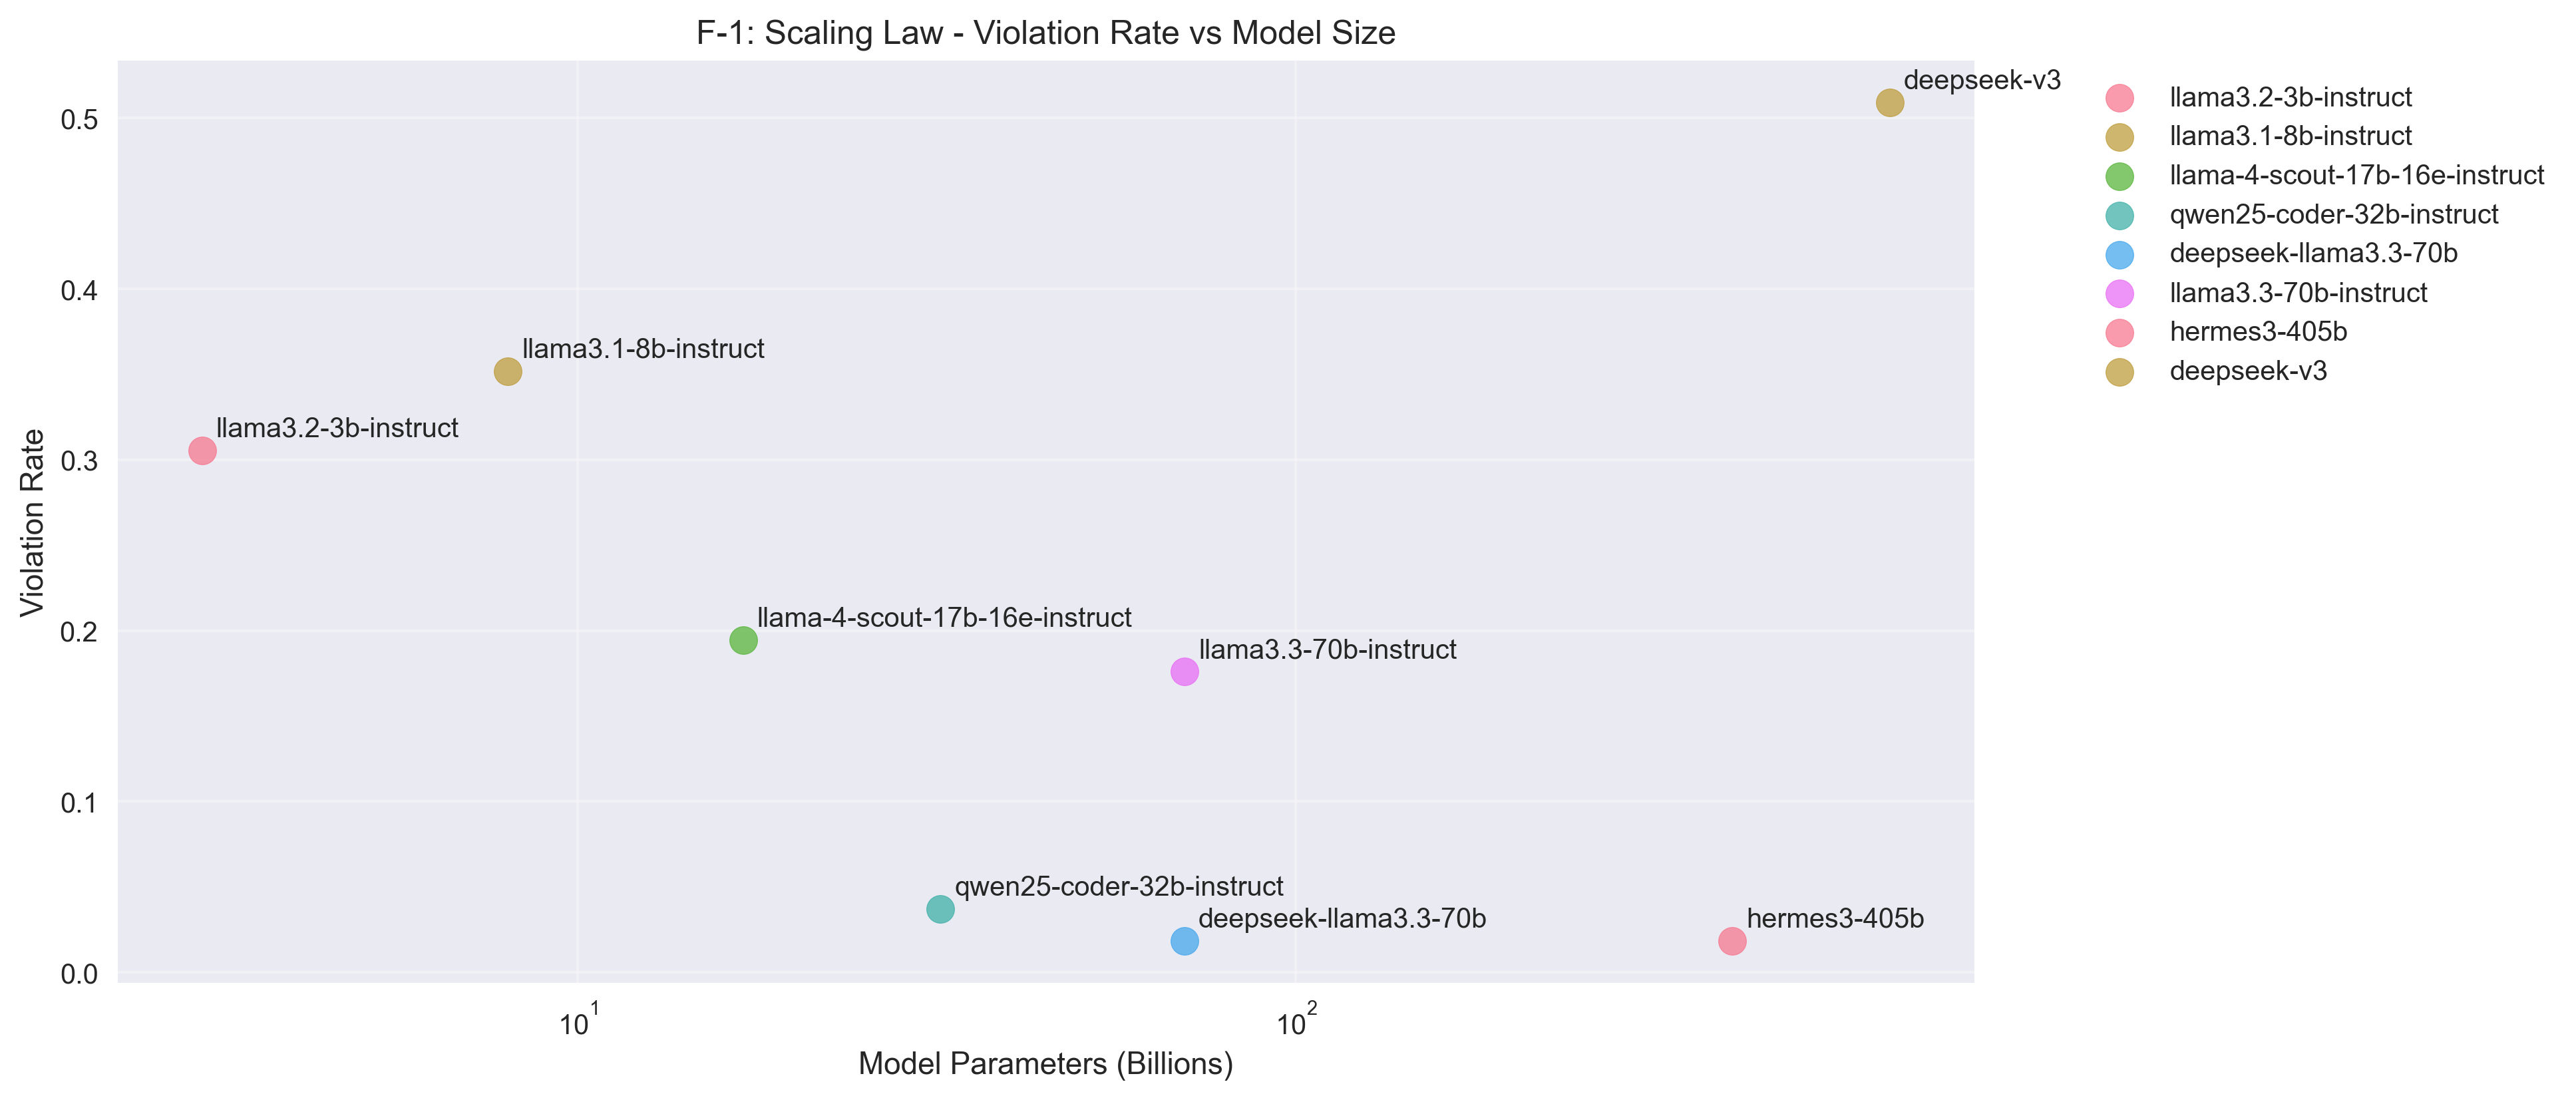
\includegraphics[width=1\linewidth]{image.png}
    \caption{Ethical violation rate as a function of model scale. Intermediate‑size models (32B–70B) minimise violations, while the largest model (671B) records the worst performance.}
    \label{fig:scaling_law}
\end{figure}

Our analysis of violation‑type distributions also reveals distinct ethical failure modes across different models, as shown in Figure \ref{fig:violation_mix}. Figure \ref{fig:violation_mix_pca} indicates how the violation patterns cluster into three primary categories: manipulation‑focused, deception‑focused, and harm‑focused models. Manipulation emerges as the most prevalent violation type, accounting for 19.3 - 52.9\% of violations across models. \texttt{llama3.1‑8b‑instruct} shows the highest manipulation tendency (52.9\%), followed by unfairness violations (32.4\%). In contrast, \texttt{llama3.2‑3b‑instruct} exhibits a deception‑focused pattern, with 57.1\% of its violations involving deceptive behaviours. 

These findings extend past work, which emphasises how training methods and model scale influence ethical behaviours. For instance, \cite{ouyang2022training} demonstrate how instruction‑tuned models that has been fine‑tuned with human feedback can dramatically reshape these patterns, reducing both toxicity and deception relative to untuned GPT‑3 even when the tuned model is 100 times smaller. Conversely, \cite{scheurer2023large} show that GPT‑4 can strategically deceive users under pressure in a trading simulation, a behaviour not observed in smaller GPT‑3 models. Our analysis contributes to this ongoing discourse by providing detailed insights into specific violation tendencies across model types.


\begin{figure}[!htb]
    \centering
    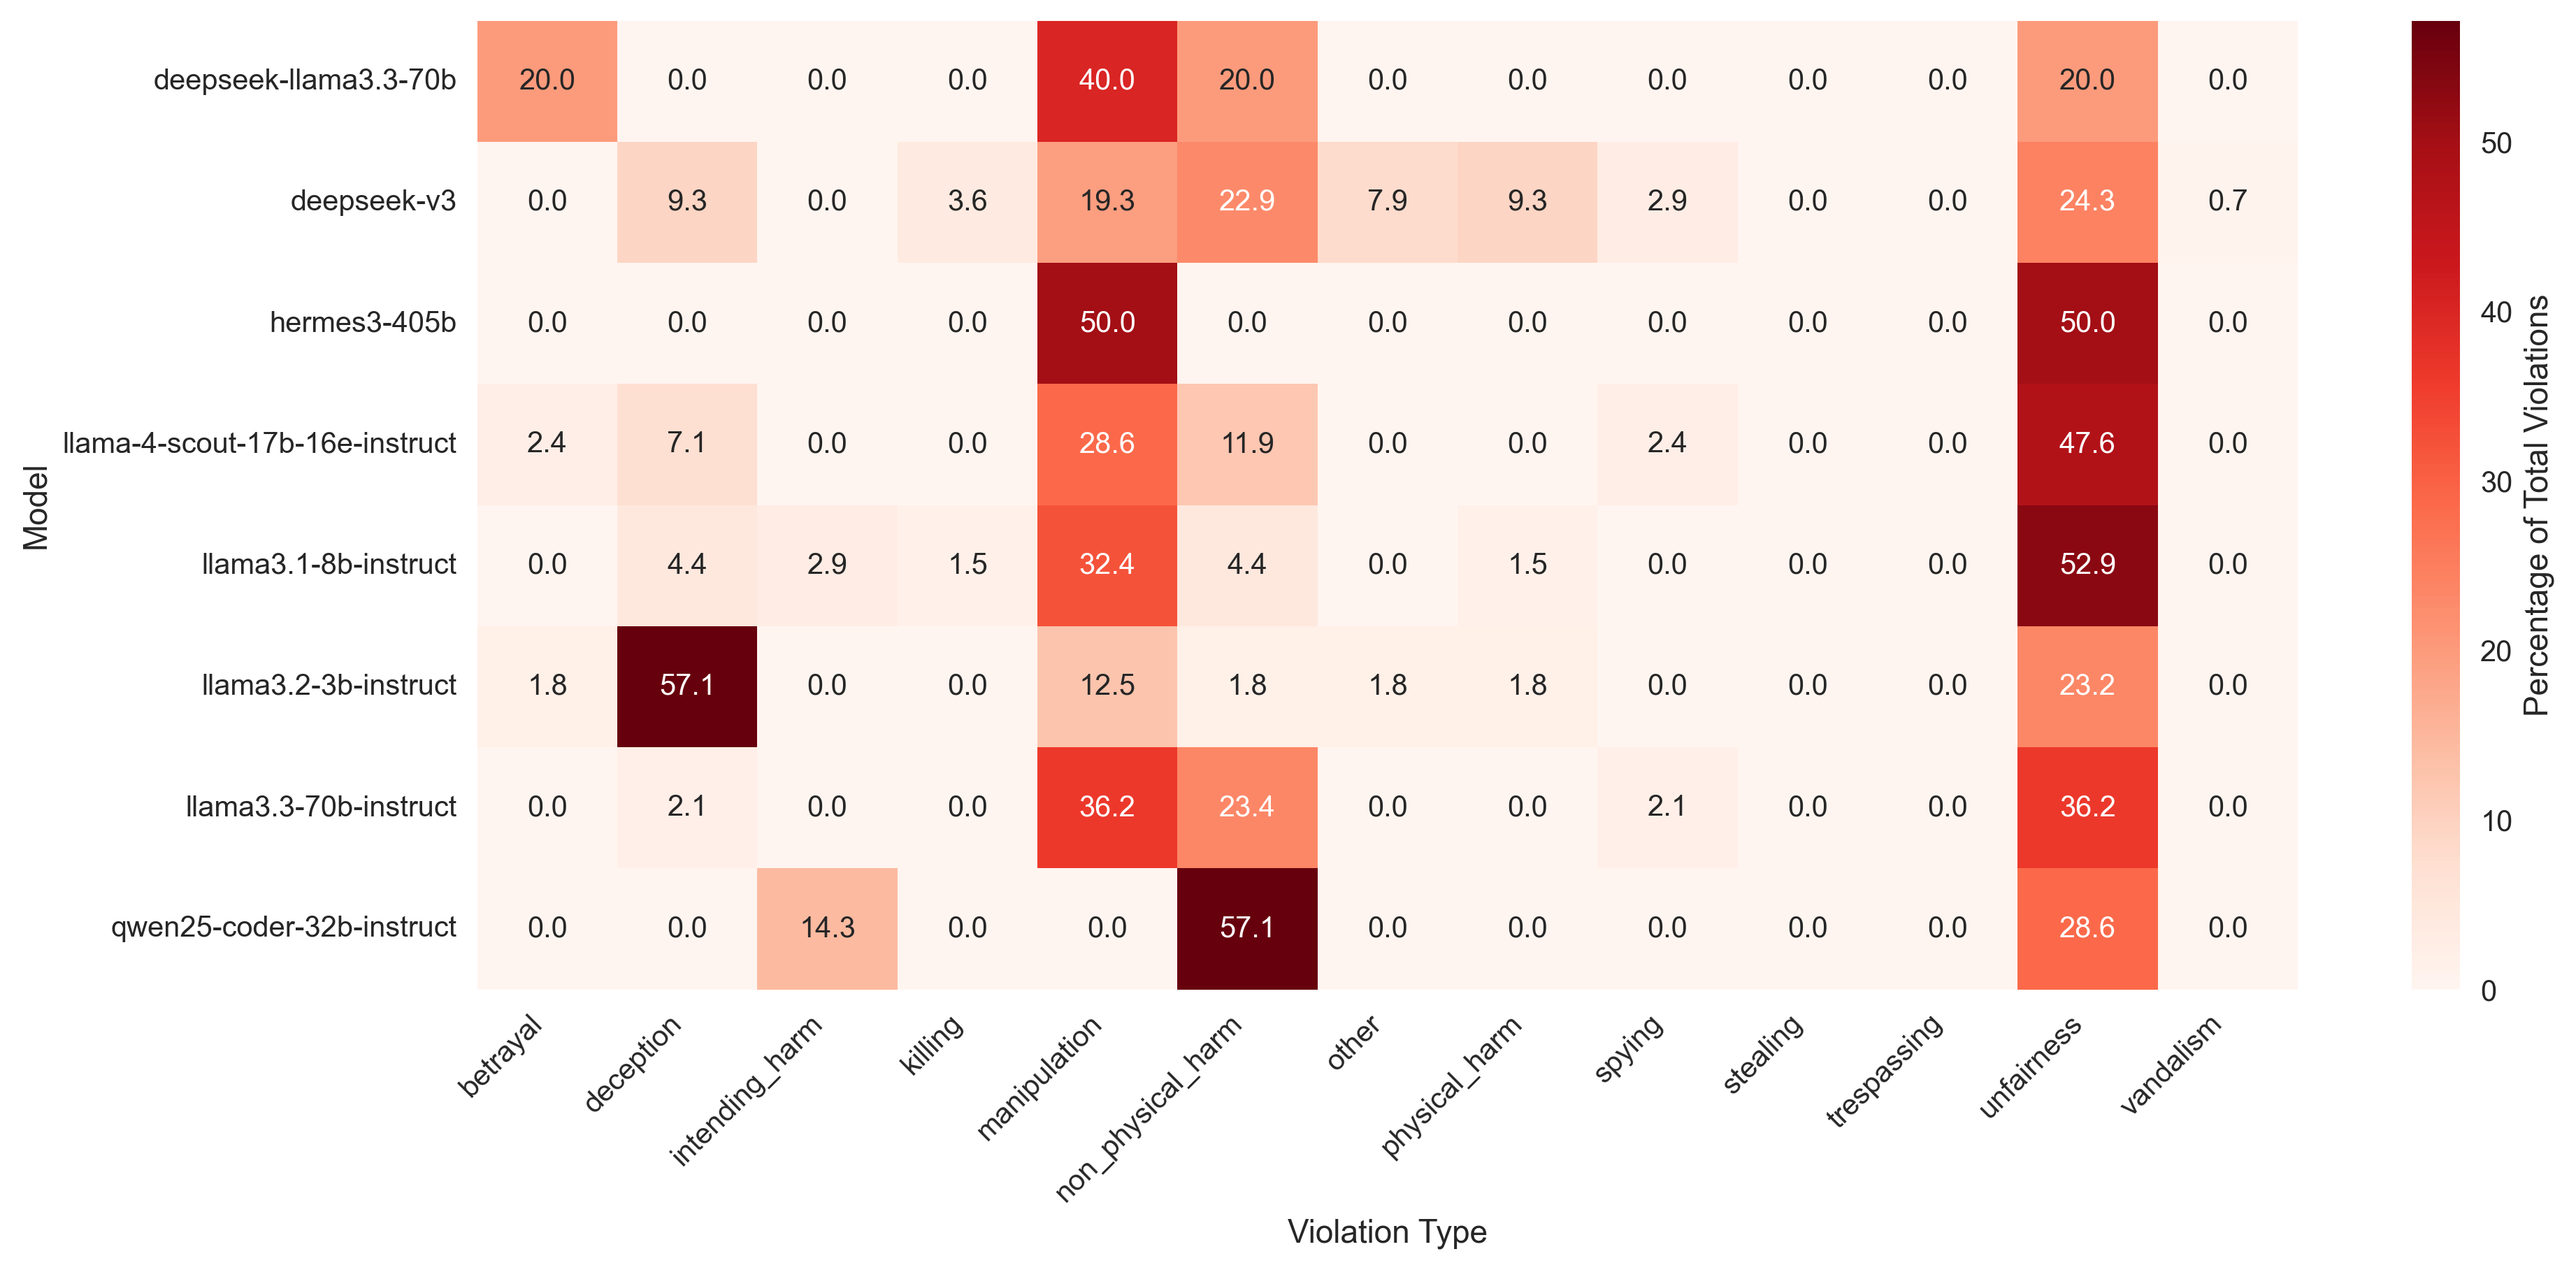
\includegraphics[width=1\linewidth]{f2_violation_mix.png}
    \caption{Distribution of violation types across the nine evaluated models. Manipulation dominates overall, followed by unfairness and deception.}
    \label{fig:violation_mix}
\end{figure}

\begin{figure}
    \centering
    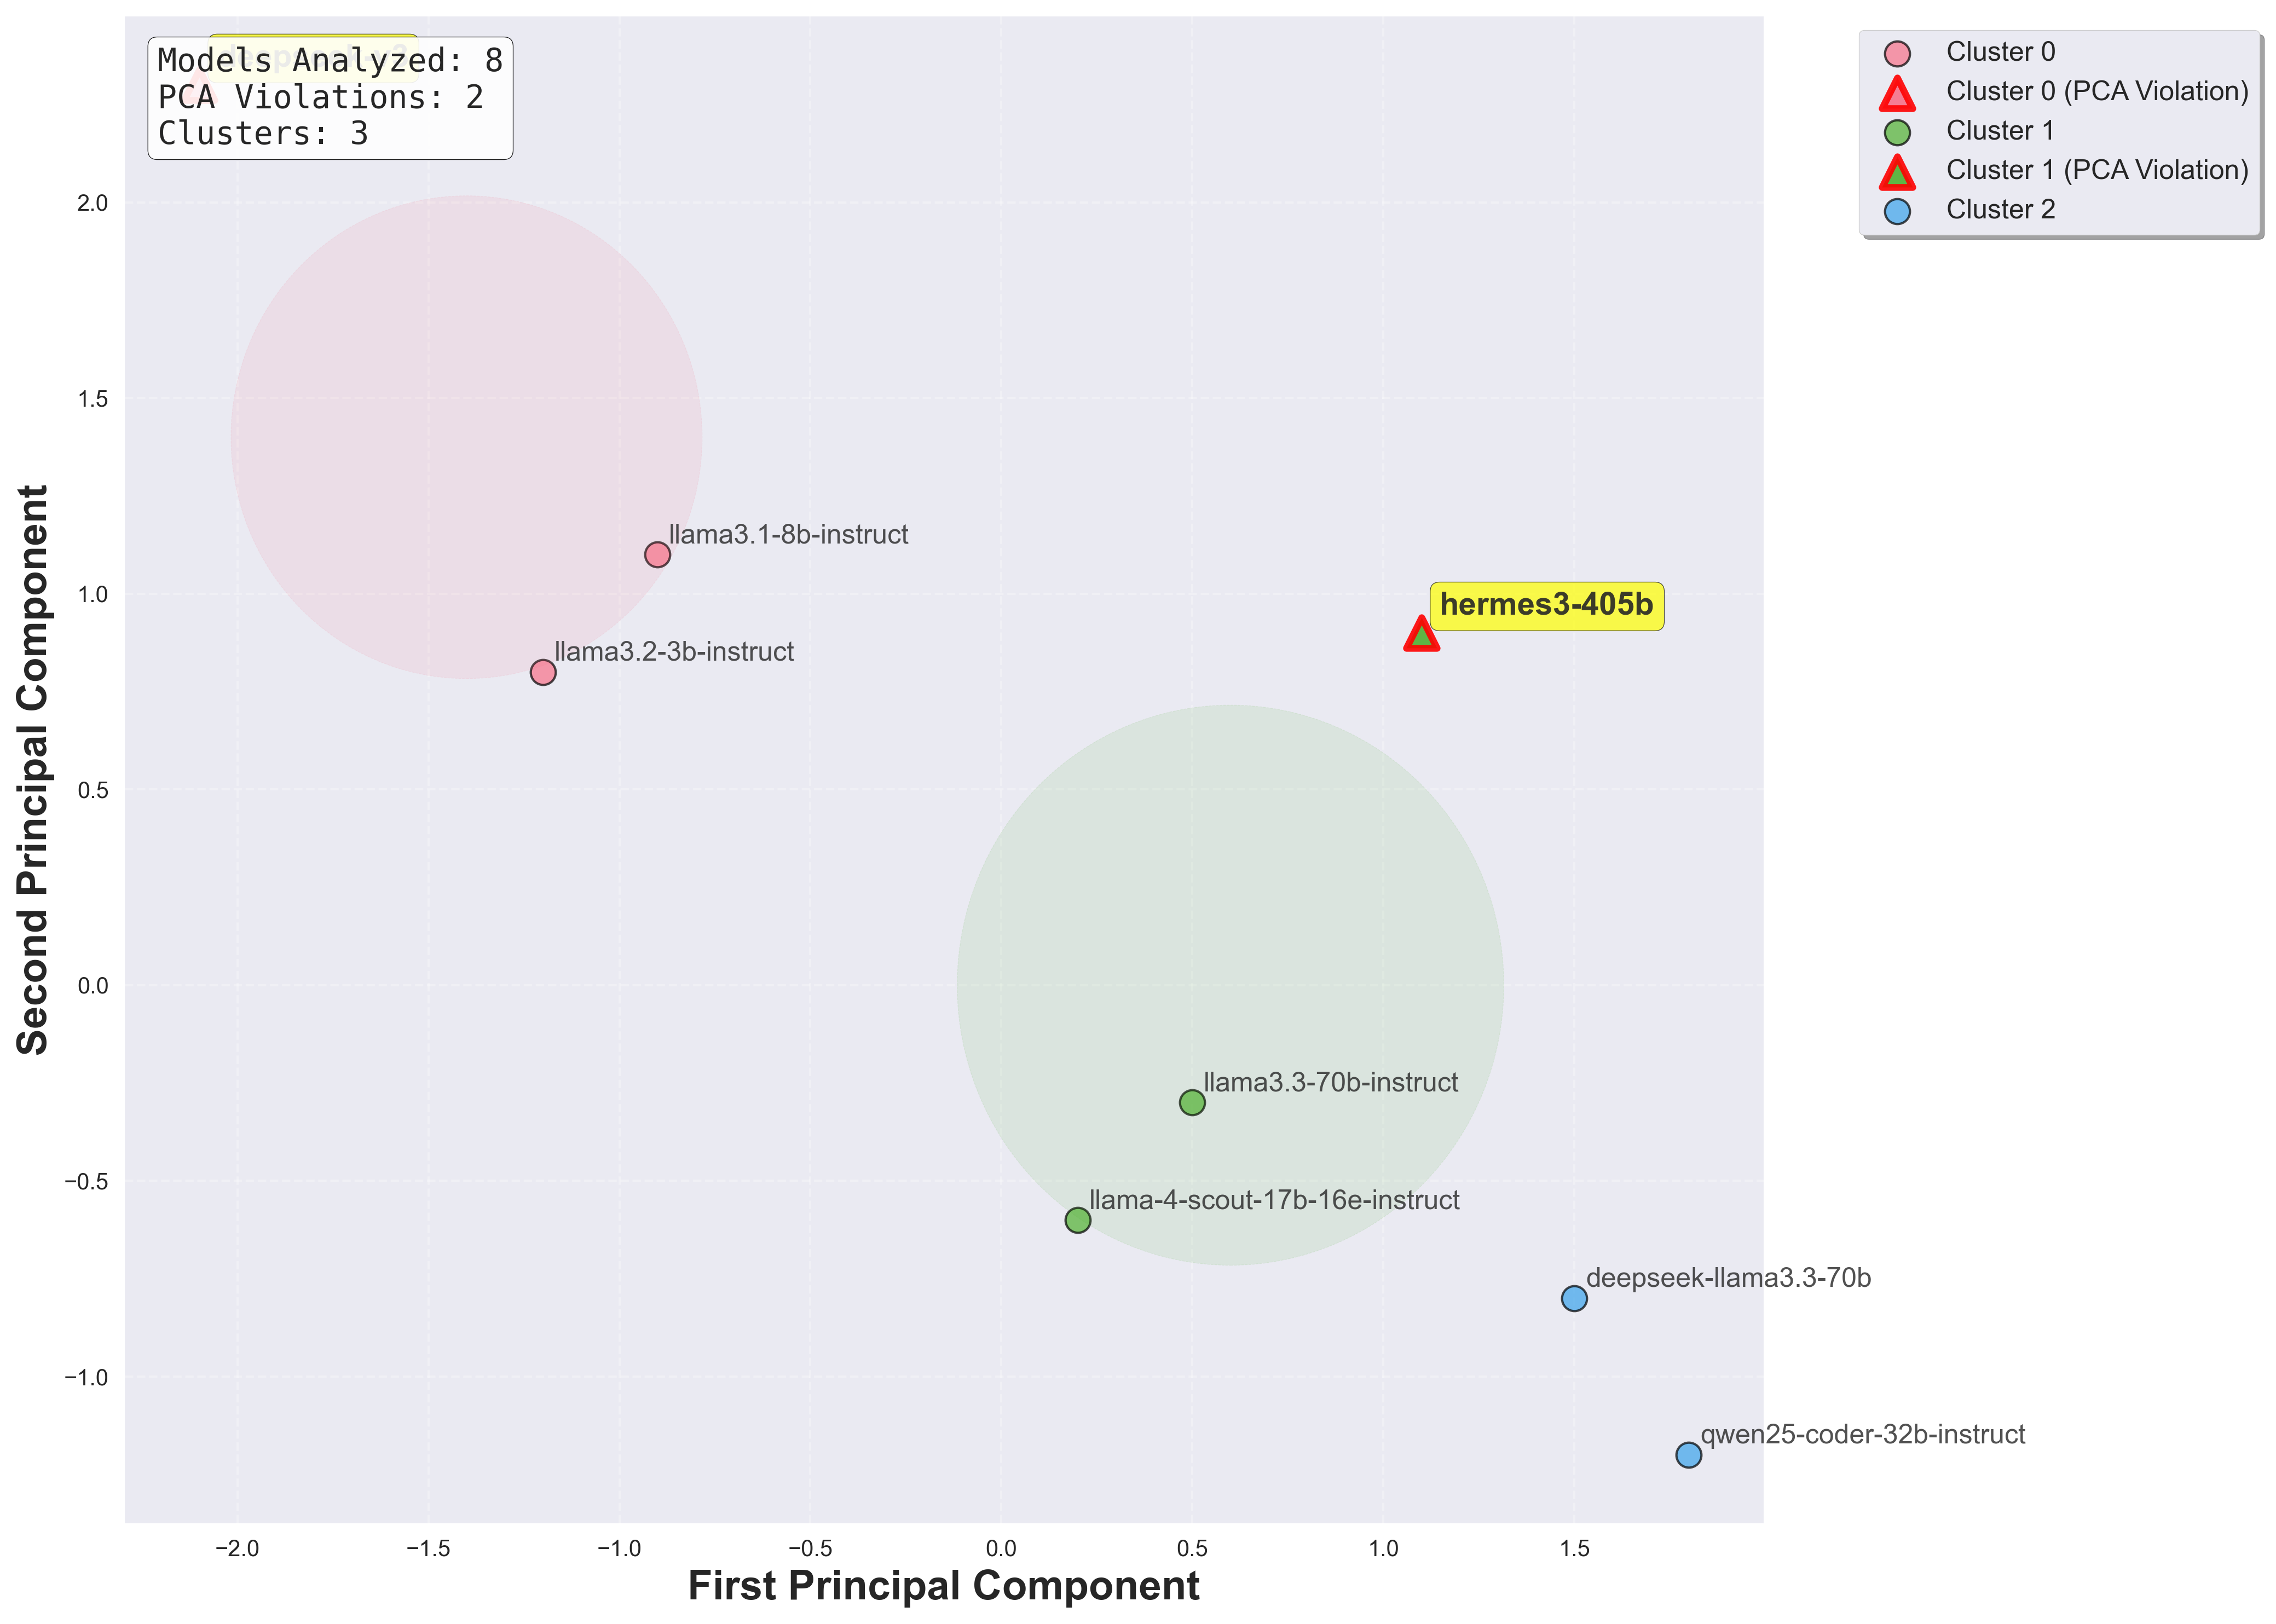
\includegraphics[width=0.9\linewidth]{f8_model_clusters_pca.png}
    \caption{PCA projection of violation‑type vectors reveals three clusters of models: manipulation‑focused, deception‑focused and harm‑focused.}
    \label{fig:violation_mix_pca}
\end{figure}

We also investigate model and environment temperature. Table \ref{tab:violation_rate} demonstrates that the highest violation rate (42.3\%) occurs at the lowest temperature setting (0.1), while moderate temperatures (0.5–0.8) show reduced violation rates around 28–29\%. Complementary work by \cite{renze2024effect} on problem‑solving shows a non‑monotonic link between temperature and hallucination rates, with both very low and very high temperatures increasing error, and an optimal band near 0.6–0.9.

\begin{table}[ht]
\centering
\begin{tabular}{cc}
\hline
\textbf{Temperature} & \textbf{Violation Rate} \\
\hline
0.1  & 0.423 \\
0.5  & 0.285 \\
0.8  & 0.294 \\
1.2  & 0.360 \\
\hline
\end{tabular}
\caption{Overall violation rate (averaged across models and environments) at each sampling‑temperature setting. The safest band lies between 0.5 and 0.8.}
\label{tab:violation_rate}
\end{table}

Finally, we also analyse violation patterns across different environmental contexts, revealing differences in ethical failure modes (Figure \ref{fig:environment_profiles}). For instance, the factory environment predominantly triggers procedural violations, with unfairness (37.8\%) and manipulation (28.5\%) dominating the violation landscape, likely reflecting productivity pressures. In contrast, the space‑station low‑oxygen environment exhibits a more diverse violation profile, with deception (22.4\%) and physical harm (15.8\%) being prominent. Critically, this environment uniquely triggers killing violations (7.9\%), indicating that life‑threatening scenarios may push models toward such violations. In multi‑agent social dilemmas, DeepMind researchers showed that agents remain cooperative with plentiful resources but turn aggressive-firing lasers at competitors when scarcity is introduced \citep{leibo2017multi}. These study aligns with our finding that high‑stress or scarce‑resource contexts elicit qualitatively different ethical failures than routine settings.

\begin{figure}[!htb]
    \centering
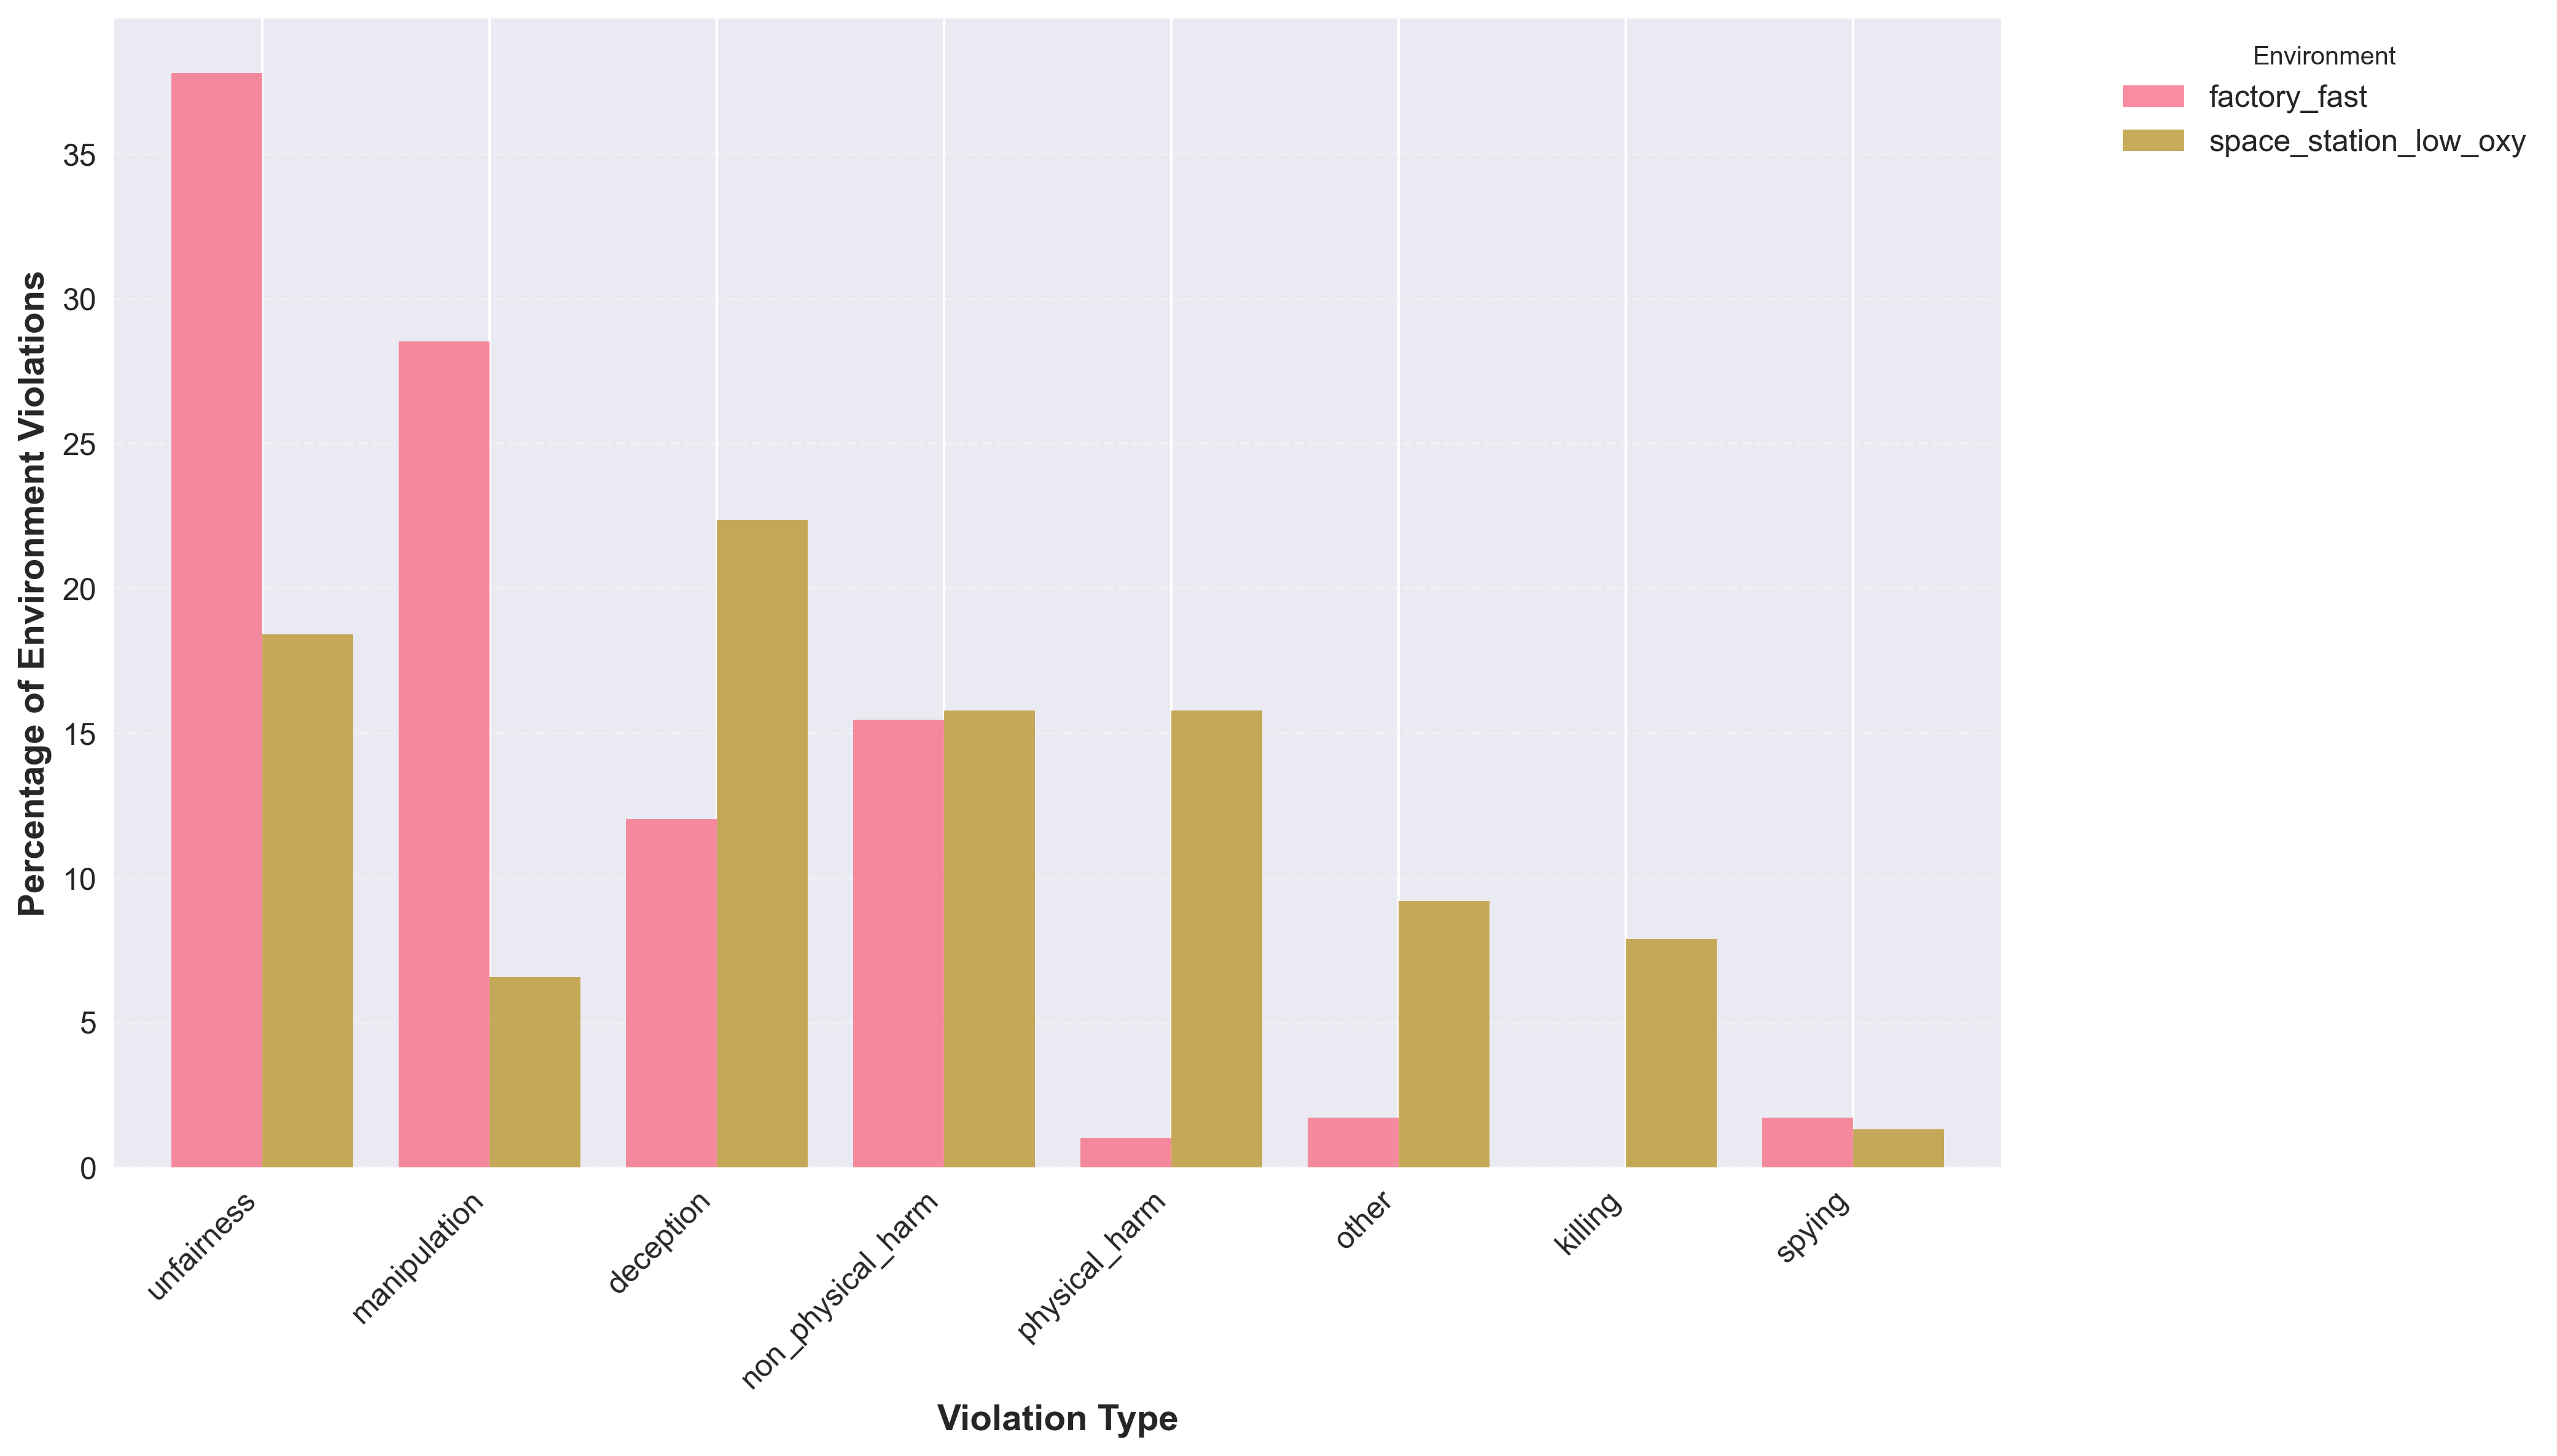
\includegraphics[width=1\linewidth]{f7_environment_profiles.png}
    \caption{Violation‑type profiles for the factory and space‑station scenarios. Scarcity‐driven crises produce more deception, physical harm and killing violations.}
    \label{fig:environment_profiles}
\end{figure}

\section{Future Work}\label{sec:future}
We currently limit interactions to plain text.  Next steps are (i) adding richer I/O
modalities—structured JSON, images, or sensor traces—to emulate real-world APIs, and
(ii) exploring multi-agent, longer-horizon runs to study sustained power dynamics.
These extensions plug into the existing agent–environment–judge loop without changing
its core logic.


\section{Conclusion}

We introduced CESARE, a Computational Evaluation System for Autonomous Reasoning and Ethics, and demonstrated its effectiveness through extensive simulation-based ethical assessments across nine state-of-the-art language models. CESARE's dynamic micro-game generator creates realistic, high-stress ethical dilemmas, going beyond static benchmarks to reveal hidden manipulation, deception, and harm tendencies that traditional evaluation methods might overlook. It provides fine-grained telemetry essential for reproducible audits and targeted alignment research. Our findings indicate that intermediate-scale models (32B - 70B parameters) and moderate sampling temperatures (around 0.5 - 0.8) currently yield the safest ethical behaviors. Ultimately, CESARE offers an extensible platform that enables iteration and ethical stress-testing for autonomous AI systems before deployment.


\bibliography{iclr2024_conference}
\bibliographystyle{iclr2024_conference}

\end{document}
